\documentclass[12pt, a4paper]{article}

% Preamble
\usepackage{xeCJK}
\usepackage[utf8]{inputenc}
\usepackage[english]{babel}
\usepackage[margin=1in]{geometry}
\usepackage[parfill]{parskip}
\usepackage{listings}
\usepackage{graphics}
\usepackage{graphicx}
\usepackage{nasm/lang}
\usepackage{nasm/style}
\usepackage{c/style}
\usepackage{go/lang}
\usepackage{go/style}
\usepackage{reil/lang}
\usepackage{llvm/lang}
\usepackage{diff/lang}
\usepackage{diff/style}
\usepackage{dot/lang}
\usepackage{dot/style}
\usepackage{float}
\usepackage[colorlinks,linkcolor=blue]{hyperref}

\usepackage{listings}
%\usepackage{color}

% Document

\usepackage{etoolbox}
\makeatletter
\def\@xobeysp{\hspace{0pt}\mbox{ }\hspace{0pt}}
\appto\verbatim@font{\hyphenchar\font`-\relax}
\apptocmd\@sverb{\hspace*{0pt}}{}{}
\makeatother

\definecolor{vgreen}{RGB}{104,180,104}
\definecolor{vblue}{RGB}{49,49,255}
\definecolor{vorange}{RGB}{255,143,102}
\lstdefinestyle{verilog-style}
{
	language=Verilog,
	basicstyle=\small\ttfamily,
	breaklines=true,
	showstringspaces=false,
	columns=flexible,
	keywordstyle=\color{vblue},
	identifierstyle=\color{black},
	commentstyle=\color{vgreen},
	numbers=left,
	numberstyle=\tiny\color{black},
	numbersep=7pt,
	tabsize=4,
	literate=*{:}{{\textcolor{black}{:}}}1
}

\title{COD\_LAB3 寄存器堆与计数器}
\author{黄业琦 PB17000144}
\date{April 7, 2019}
\begin{document}
\maketitle
\tableofcontents
\clearpage
\section{实验目的}
\subsection{寄存器堆(Register File)}
ra0, rd0; ra1, rd1:2个异步读端口\\
wa, wd, we:1个同步写端口
\subsection{计数器(Counter)}
ce:计数使能,1: q=q+1\\
pe:同步装数使能,1: q=d\\
rst:异步清零,1: q=0
\begin{figure}[H]
	\centering
	\includegraphics[width=0.35\linewidth]{Req1}
	\includegraphics[width=0.5\linewidth]{Req2}
	\caption{Lab Requirement}
	\label{fig:req}
\end{figure}

\subsection{FIFO}
最大长度为8的FIFO循环队列:用寄存器堆和适当逻辑实现。\\
en\_out, en\_in:出/入队列使能,一次有效仅允许操作一项数据\\
out, in:出/入队列数据\\
full, empty:队列空/满,空/满时忽略出/入队操作\\
display:8个数码管的控制信号,显示队列状态

\section{实验环境}
Linux下编程调试和仿真,使用IVerilog,GtkWave系列工具。\\
Windows下用于生成比特流文件,使用Vivado 2018.2,Verilog HDL\\
所有下载均在Nexsy4-DDR实验板完成

\section{逻辑设计}
\subsection{Regfile Design}
两个地址读入位置,直接用有带宽的向量作为存储寄存器。我们直接访问对应位置的元素进行访问即可。
\subsection{Counter Design}
计数器,设计简单,与上学期的lab8,9一致,不再赘述。
\subsection{FIFO\_q Design}
FIFO设计:\\
我并没有单独调用我自己设计的Regfile,因为队列的特殊性,我决定直接设计有带宽的向量组直接使用。\\
这样大大降低了编程的复杂程度。\\
计数器我则用于分频,分八个段供八个七段数码管使用。\\
由于传向量组并不是Verilog的合法语法,有两种解决办法:
\begin{enumerate}
	\item 避免调用,合并程序。
	\item 压缩向量,变为1维。
\end{enumerate}
权衡选择第一种。入队出队操作见示意图:\\
\begin{figure}[H]
\centering
\includegraphics[width=0.9\linewidth]{FIFOshow1}
\caption{fifoshow1}
\label{fig:fifoshow1}
\end{figure}
\begin{figure}[H]
\centering
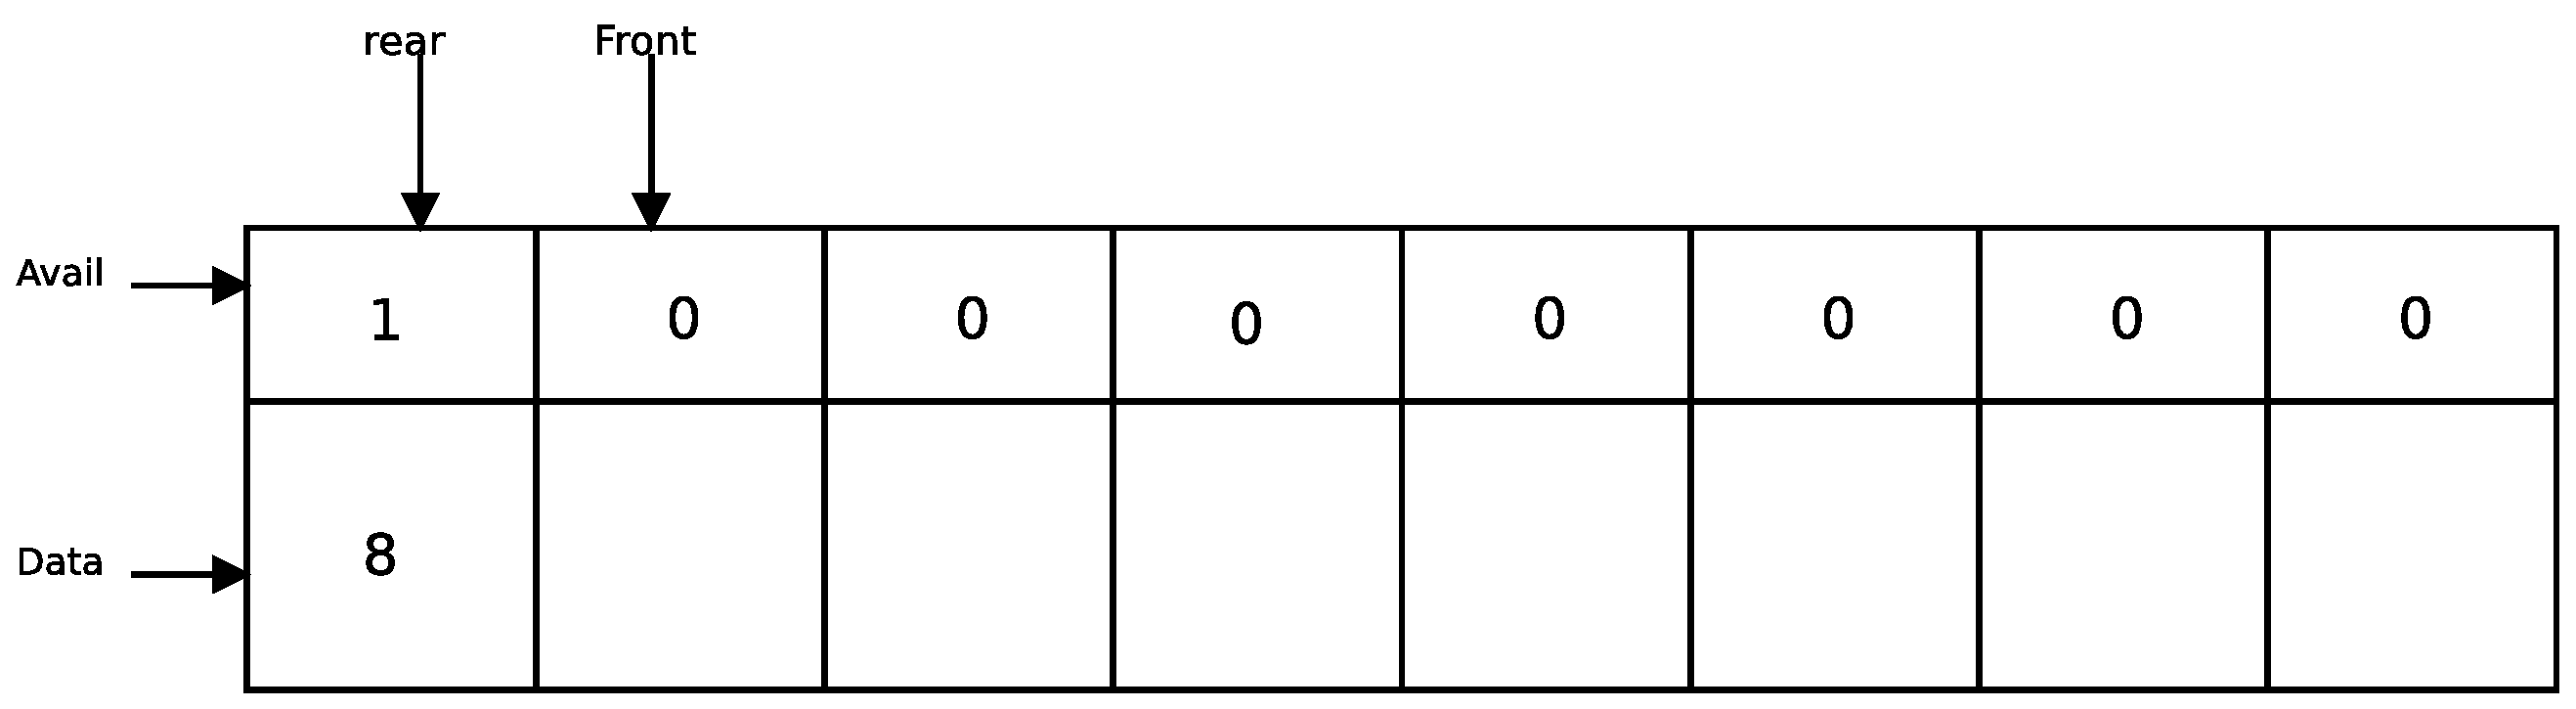
\includegraphics[width=0.9\linewidth]{FIFOshow2}
\caption{fifoshow2}
\label{fig:fifoshow2}
\end{figure}
\begin{figure}[H]
\centering
\includegraphics[width=0.9\linewidth]{FIFOshow3}
\caption{fifoshow3}
\label{fig:fifoshow3}
\end{figure}
front指向对头后一个元素,rear指向队尾元素。
\clearpage
\section{仿真截图}
\begin{figure}[H]
	\centering
	\includegraphics[width=0.9\linewidth]{Regsim}
	\caption{Regsim}
	\label{fig:Regsim}
\end{figure}

\begin{figure}[H]
	\centering
	\includegraphics[width=0.9\linewidth]{Countsim}
	\caption{Countsim}
	\label{fig:Countsim}
\end{figure}

\begin{figure}[H]
\centering
\includegraphics[width=0.9\linewidth]{FIFOsim}
\caption{FIFOsim}
\label{fig:FIFOsim}
\end{figure}
\clearpage
\section{性能评测截图}
\begin{figure}[H]
	\centering
	\includegraphics[width=0.9\linewidth]{Regper1}
	\caption{Regper1}
	\label{fig:Regper1}
\end{figure}

\begin{figure}[H]
	\centering
	\includegraphics[width=0.9\linewidth]{Regper2}
	\caption{Regper2}
	\label{fig:Regper2}
\end{figure}

\begin{figure}[H]
	\centering
	\includegraphics[width=0.9\linewidth]{Countper1}
	\caption{Countper1}
	\label{fig:Countper1}
\end{figure}

\begin{figure}[H]
	\centering
	\includegraphics[width=0.9\linewidth]{Countper2}
	\caption{Countper2}
	\label{fig:Countper2}
\end{figure}

\begin{figure}[H]
	\centering
	\includegraphics[width=0.9\linewidth]{FIFOper1}
	\caption{FIFOper1}
	\label{fig:FIFOper1}
\end{figure}

\begin{figure}[H]
	\centering
	\includegraphics[width=0.9\linewidth]{FIFOper1}
	\caption{FIFOper1}
	\label{fig:FIFOper1}
\end{figure}
\clearpage
\section{实验代码}
\subsection{Regfile 代码}
\lstinputlisting[style={verilog-style},caption={Regfile.v}]{/home/chivier_humber/Desktop/Study/COD_LAB/LAB3/Regfile/Regfile.srcs/sources_1/new/Regfile.v}
\lstinputlisting[style={verilog-style},caption={RegSim.v}]{/home/chivier_humber/Desktop/Study/COD_LAB/LAB3/Regfile/Regfile.srcs/sim_1/new/RegSim.v}
\subsection{Counter 代码}
\lstinputlisting[style={verilog-style},caption={counter.v}]{/home/chivier_humber/Desktop/Study/COD_LAB/LAB3/Count/Count.srcs/sources_1/new/counter.v}
\lstinputlisting[style={verilog-style},caption={counter\_tb.v}]{/home/chivier_humber/Desktop/Study/COD_LAB/LAB3/Count/Count.srcs/sim_1/new/counter_tb.v}
\subsection{FIFO 代码}
这里的注释部分为调试使用,代码的36-41行的取消注释,54行取消注释,47行换为46行,可以进行仿真。
\lstinputlisting[style={verilog-style},caption={clk10HZ.v}]{/home/chivier_humber/Desktop/Study/COD_LAB/LAB3/FIFO/FIFO.srcs/sources_1/new/clk10HZ.v}
\lstinputlisting[style={verilog-style},caption={BCD27.v}]{/home/chivier_humber/Desktop/Study/COD_LAB/LAB3/FIFO/FIFO.srcs/sources_1/new/BCD27.v}
\lstinputlisting[style={verilog-style},caption={counter.v}]{/home/chivier_humber/Desktop/Study/COD_LAB/LAB3/FIFO/FIFO.srcs/sources_1/new/counter.v}
\lstinputlisting[style={verilog-style},caption={FIFO.v}]{/home/chivier_humber/Desktop/Study/COD_LAB/LAB3/FIFO/FIFO.srcs/sources_1/new/FIFO.v}
\lstinputlisting[style={verilog-style},caption={FIFO\_tb.v}]{/home/chivier_humber/Desktop/Study/COD_LAB/LAB3/FIFO/FIFO.srcs/sim_1/new/FIFO_tb.v}
\end{document}
